\subsection{Filtered data points match C}
\label{sec:filteredDataPointsMatchC}

Running the outlined program in Gezel yields the results shown in figure \ref{fig:CvsGezel}. As seen in the figure, the results in C (using $N=32$) and results from the hardware implementation match perfectly, i.e. the 250 sets of filtered data points (C vs. Gezel) differ by 0.
%As seen in the figure, the expected results from a division by 32 instead of by 30, matches the output from the hardware implementation perfectly. This means, that our implementation and CPU work as expected. 

\begin{figure}[H]
\centering
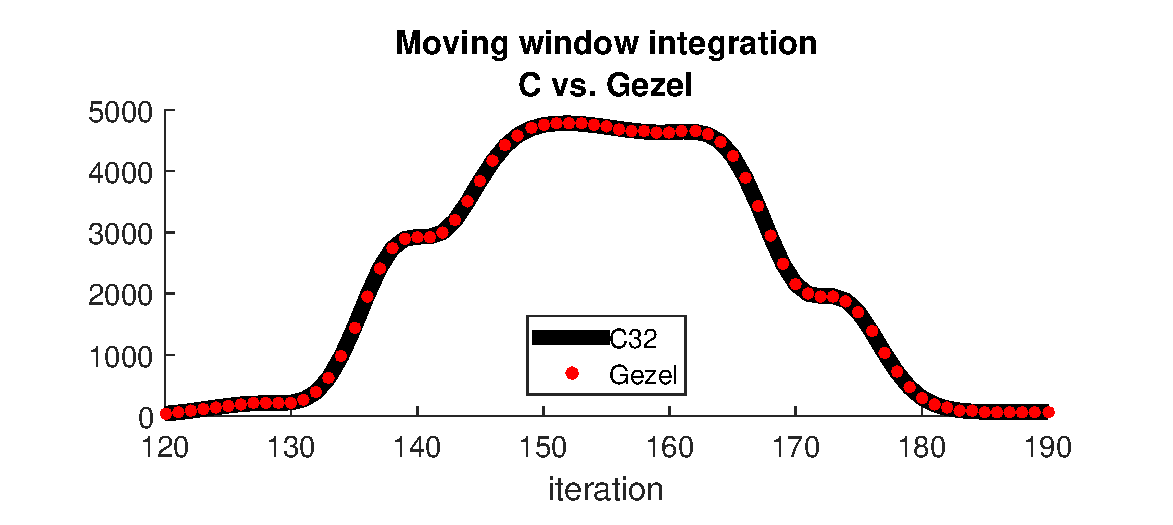
\includegraphics[width=1.0\textwidth]{3Results/fig/CvsGezel.eps}
\caption{Comparing the filtered data Gezel and C (using $N=32$). The data points are exact matches for the first 250 data points.}
\label{fig:CvsGezel}
\end{figure}

This means that our implementation and CPU work as expected, and that is indeed possible to implement the moving window integration filter in Gezel. Whether it is reasonable depends on the performance; is the hardware implementation fast enough? Does the speed gained from implementing the filter in hardware outweigh the speed lost by communicating between software and hardware? Does it consume less energy?
